\section{Experimental Results}
% Select Ransac, because we are not sure that more than half of the keypoints are inliers
The first part of this section presents the result of RANSAC for homography estimation by identifying outliers. While LMS method (section~\ref{sec:least-median-square}) works good when there are more than 50\% inliers, it is not always guaranteed to have more than half accurate matches\footnote{there might be chances of being more false matches since we have used less accurate methods like SURF and ANN to get faster result}, so I prefer RANSAC method for robust estimation and it works even if there are large number of outliers. The equation~\ref{eq:number-of-iterations} reveals that we need few iterations to get a pure sample with high probability even if there are a lot of outliers.\\

\noindent In the next section, I include experiment on the effect of distance threshold value ($\sigma$) to the number of inliers or outliers.  The distance threshold $\sigma$ has been measured in pixels. 

\subsection{Robust Estimation with RANSAC}
For RANSAC, I have set the maximum possible number of iterations ($N$) up to 2000 and distance threshold ($\sigma$) 2 pixels. After some iterations, I got inliers (accurate matches), outliers (inaccurate matches) and the homography matrix $H$. Figure~\ref{fig:RANSAC-result} shows the inlier matches after I obtained using RANSAC method. From the figure, we can easily see that the all inliers are true matches.

\begin{figure}[H]%
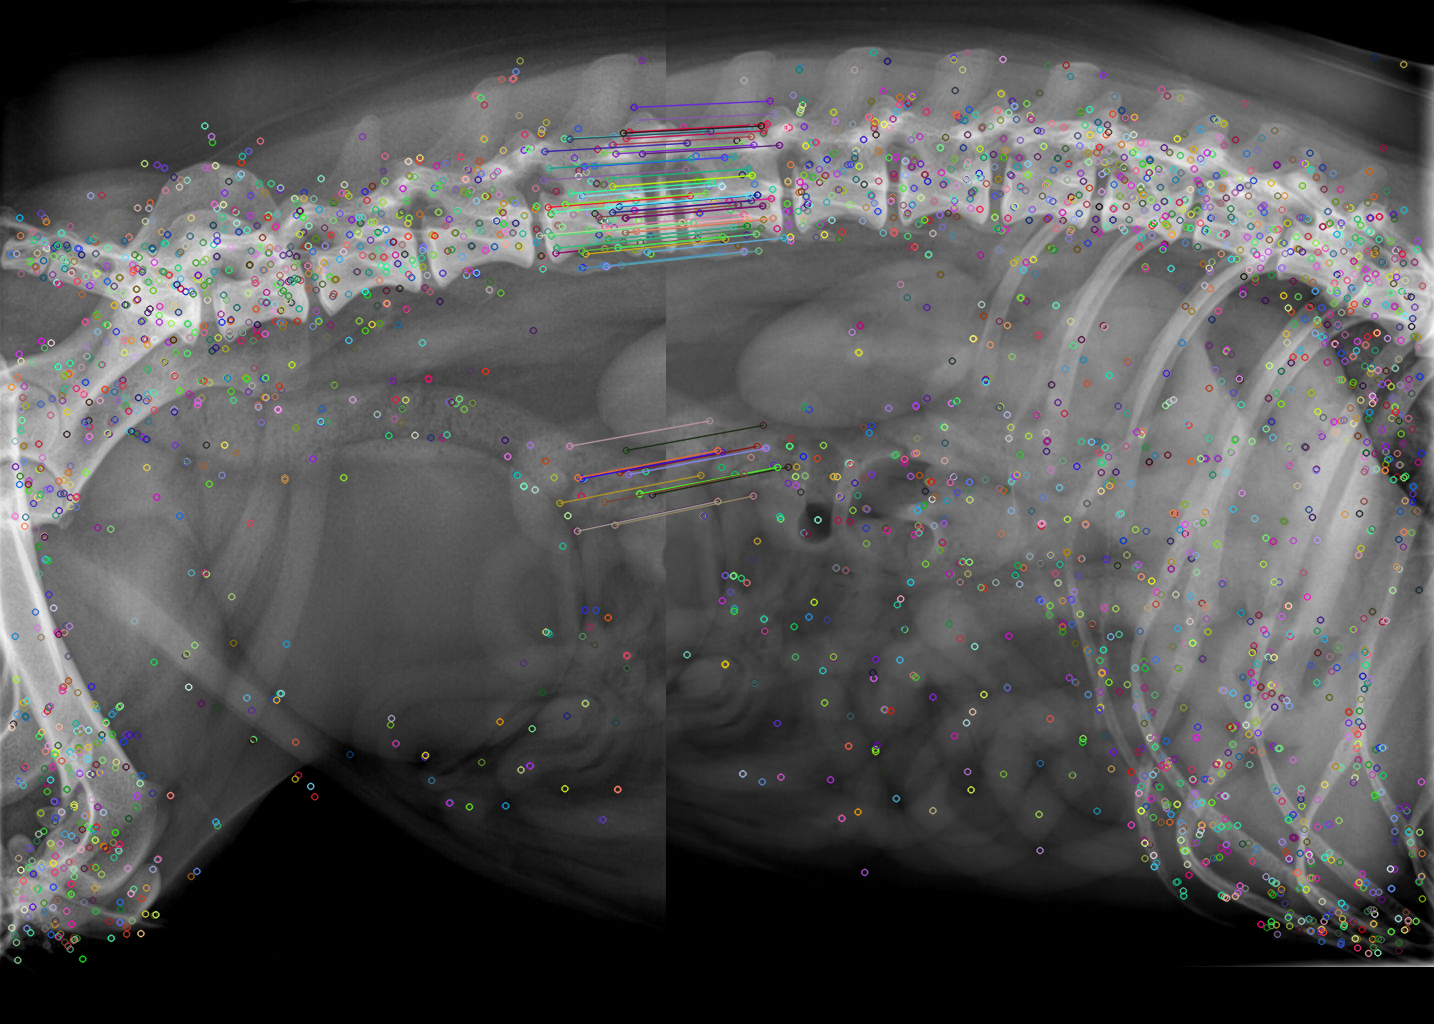
\includegraphics[scale=0.25]{2.mainmatter/2.Methodology/figures/inliers}
\caption[Matches After Removing Outliers]{Matches after removing outliers ($\sigma$=3 pixels). This figure shows all matches are accurate.}%
\label{fig:RANSAC-result}%
\end{figure}

\subsection{Effect of Distance Threshold ($\sigma$)}
The number of inliers is changed when we change the distance threshold $\sigma$. This section includes experiment on the effect of $\sigma$ to the number of inliers we obtained. The graph presented in figure~\ref{fig:inliers-vs-distance-threshold} shows that increase of $\sigma$, increases the number of inliers. So, we have to select proper $\sigma$ so that all inliers are true matches. With small possible value of $\sigma$=1 pixel, I got 50 inliers. Since the figure~\ref{fig:RANSAC-result} shows there are 62 accurate matches which implies that $\sigma$ = 1 is missing some true matches. The increase of $\sigma$ increases the inliers which also increases probability of including false matches as inliers. So, the best accepted values of $\sigma$ seems to be either 1 or 2. 

\begin{figure}[H]%
\centering
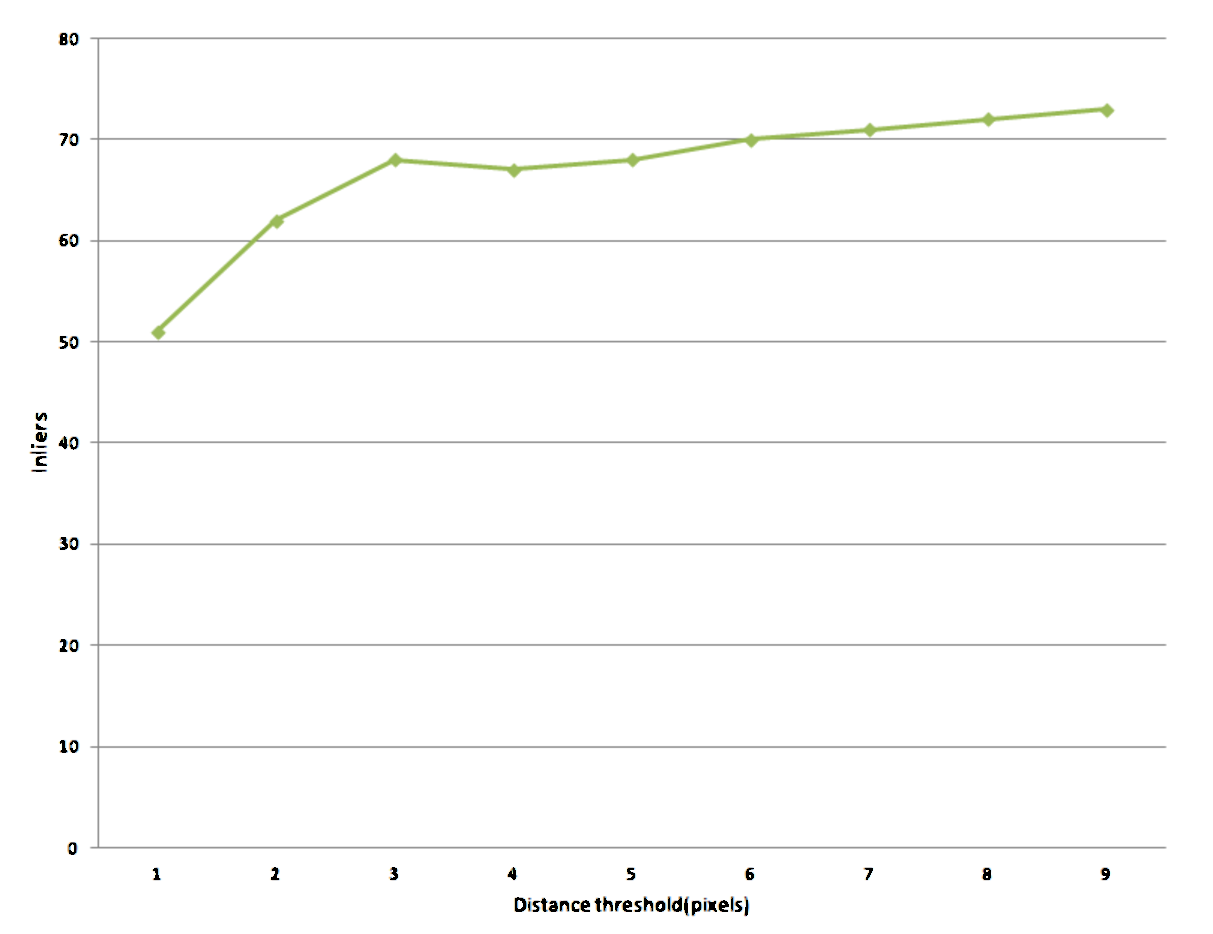
\includegraphics[width=1.0\columnwidth]{2.mainmatter/2.Methodology/figures/Inliers-threshold}%
\caption[Distance Threshold and Inliers Count]{Graph showing inliers versus distance threshold}%
\label{fig:inliers-vs-distance-threshold}%
\end{figure}

\noindent In some cases, if the stitching X-ray images are not exactly same, then key-points do not go with the transformation model (i.e. $H$) which results very few or sometimes insufficient inliers to guarantee the accuracy of homography. In that situation, we increase $\sigma$ value to get more inliers while estimating homography.\\

\noindent The number of inliers \footnote{The inliers in this context is the best inliers we got after a number of iterations.} can also be used to identify the feasibility of stitching between two images. There might be cases when we try stitching images which do not have any common region. The inliers are counted to confirm whether the images can be stitched. We define any number greater than sample size. Most of the time, if we have more than 15 inliers, we accept the homography to create composite image. For very few inliers\footnote{Few inliers imply limited or no overlapping between input images.}, there is chances of getting inaccurate homography and we stop the stitching process.

